\chapter{De cel: eenheid van het leven}\label{ch:b1:cell-unit-of-life}

In 1665 legde Robert Hooke een schilfertje kurk onder een lens en zag het
verdeeld in kleine kamertjes die hij \omterm{def:b1:cell-unit-of-life:cell}{cellen} noemde, naar de kamers van een
klooster. Tien jaar later zag een Delftse lakenhandelaar, Antoni van
Leeuwenhoek, die zijn eigen lenzen slepen tot een sterkte die niemand anders
haalde, levende wezens zwemmen in een druppel slootwater, in het schraapsel van
zijn tanden en in zijn eigen zaad. Het duurde nog anderhalve eeuw om te
verwoorden wat die twee hadden gezien: dat elk \omterm{def:b1:organism-environment:organism}{organisme} uit \omterm{def:b1:cell-unit-of-life:cell}{cellen} bestaat, en
dat elke \omterm{def:b1:cell-unit-of-life:cell}{cel} uit een \omterm{def:b1:cell-unit-of-life:cell}{cel} voortkomt. Dit hoofdstuk formuleert de \omterm{prop:b1:cell-unit-of-life:theory}{celtheorie} met
haar bewijsmateriaal, stelt de twee typen \omterm{def:b1:cell-unit-of-life:cell}{cel} tegenover elkaar, en beschrijft
de instrumenten --- de microscopen, de centrifuge, de kweekfles --- waarmee wij
\omterm{def:b1:cell-unit-of-life:cell}{cellen} kunnen zien, uit elkaar halen en buiten een \omterm{def:b1:organism-environment:organism}{organisme} in leven houden.

\section{De celtheorie}

\begin{definition}[Cel]\label{def:b1:cell-unit-of-life:cell}
Een \emph{cel}\index{cel} is de kleinste eenheid van levende materie: een
volume waterig \emph{cytoplasma}\index{cytoplasma} begrensd door een
\emph{plasmamembraan}\index{plasmamembraan}, met daarin het erfelijk materiaal
(DNA) en de machinerie die het tot uitdrukking brengt, in staat om
voedingsstoffen op te nemen, energie om te zetten, haar eigen ordening in stand
te houden en, wanneer de omstandigheden het toelaten, in twee cellen te delen.
\end{definition}

\begin{proposition}[De celtheorie]\label{prop:b1:cell-unit-of-life:theory}
\index{celtheorie}
\begin{enumerate}
  \item Elk \omterm{def:b1:organism-environment:organism}{organisme} bestaat uit één of meer \omterm{def:b1:cell-unit-of-life:cell}{cellen}, en de \omterm{def:b1:cell-unit-of-life:cell}{cel} is de
        eenheid van bouw en werking van levende wezens
        (Schleiden en Schwann, 1838--1839).
  \item Elke \omterm{def:b1:cell-unit-of-life:cell}{cel} ontstaat door deling uit een reeds bestaande \omterm{def:b1:cell-unit-of-life:cell}{cel}
        (Virchow, 1855: \emph{omnis cellula e cellula}); er is geen
        spontane generatie.
  \item Het erfelijk materiaal wordt bij de deling van \omterm{def:b1:cell-unit-of-life:cell}{cel} op \omterm{def:b1:cell-unit-of-life:cell}{cel}
        doorgegeven, zodat de continuïteit van het leven de continuïteit
        van \omterm{def:b1:cell-unit-of-life:cell}{cellen} is.
\end{enumerate}
\end{proposition}
\begin{proof}[Bewijsmateriaal]
De kurk van Hooke (1665) en de plantendoorsneden van Grew en Malpighi toonden
plantenweefsels als rijen kamertjes; de lenzen van Leeuwenhoek (jaren 1670)
toonden eencellige \omterm{def:b1:organism-environment:organism}{organismen}, bloedcellen en zaadcellen. Twee eeuwen van steeds
betere lenzen vonden \omterm{def:b1:cell-unit-of-life:cell}{cellen} in elk onderzocht \omterm{def:b1:body-plans-tissues:tissue}{weefsel}, dierlijk zowel als
plantaardig, zodra Schwann \omterm{def:b1:cell-unit-of-life:cell}{cellen} met een kern herkende in kraakbeen en embryo's.
De deling werd rechtstreeks waargenomen bij algen en in embryo's, en Virchow vond
geen enkel \omterm{def:b1:body-plans-tissues:tissue}{weefsel}, gezond of ziek, waarvan de \omterm{def:b1:cell-unit-of-life:cell}{cellen} niet uit andere \omterm{def:b1:cell-unit-of-life:cell}{cellen}
kwamen. De zwanenhalskolven van Pasteur (1861) --- bouillons die maandenlang
steriel bleven zolang stof ze niet kon bereiken, en binnen enkele dagen krioelden
zodra dat wel kon --- sloten de kwestie van de spontane generatie af. De derde
uitspraak is het werk van de late negentiende eeuw, die de chromosomen door de
deling heen volgde (\cref{ch:b1:replication-mitosis}).
\end{proof}

\begin{omfigure}
\begin{minipage}[b]{0.46\linewidth}\centering
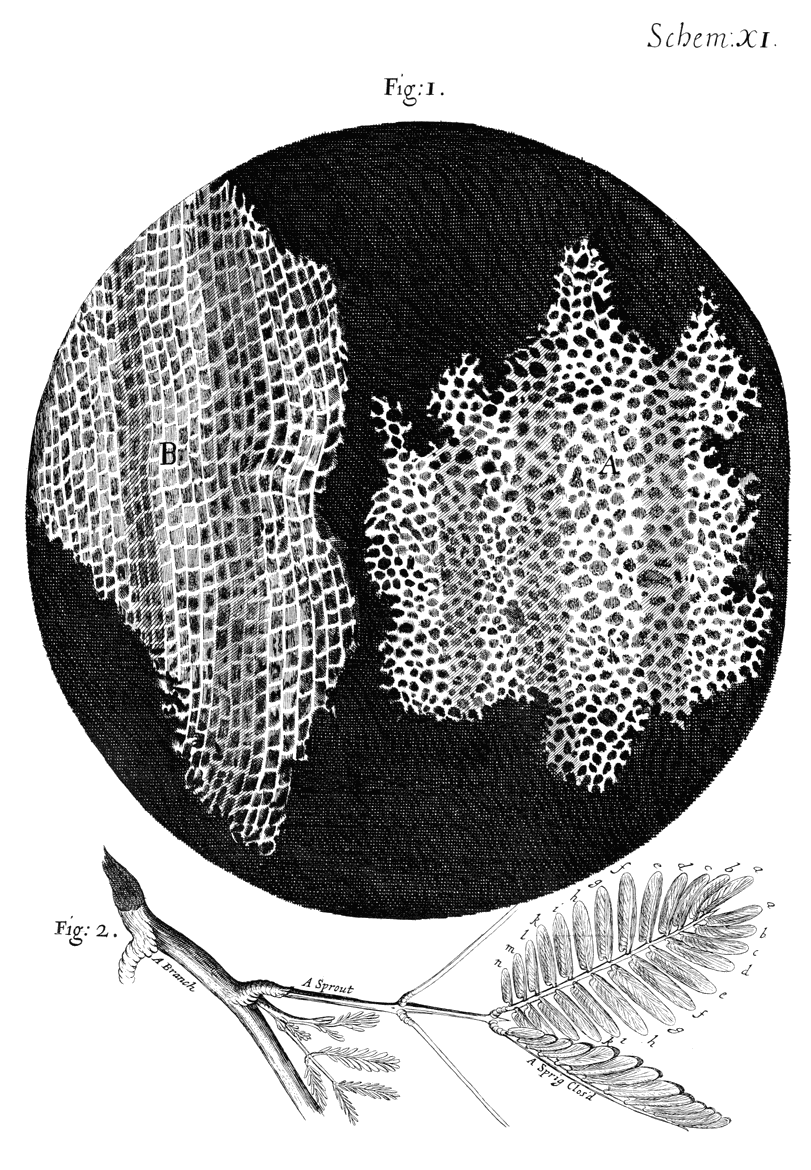
\includegraphics[width=0.9\linewidth]{images/book3/hooke-cork.png}
\end{minipage}\hfill
\begin{minipage}[b]{0.46\linewidth}\centering
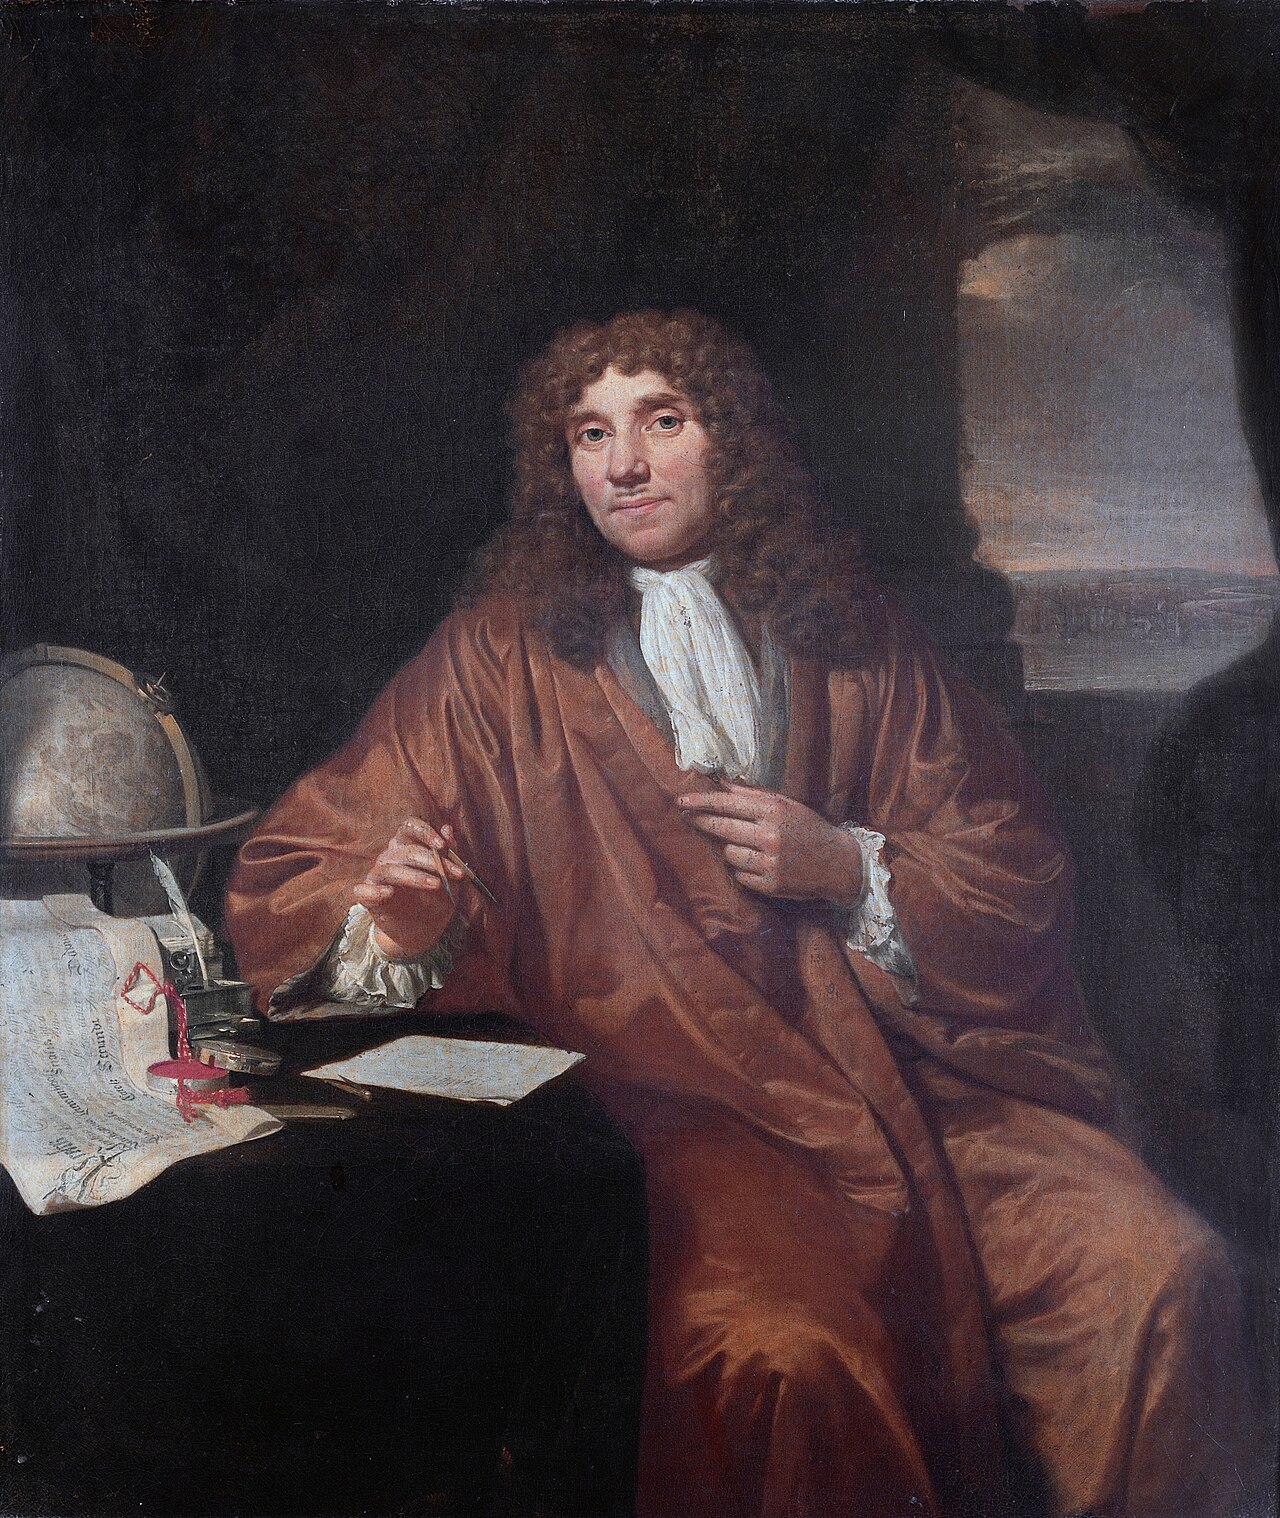
\includegraphics[width=0.78\linewidth]{images/book3/leeuwenhoek.jpg}
\end{minipage}

{\small Links: de tekening die Hooke in \emph{Micrographia} (1665) van kurk
maakte, de eerste \omterm{def:b1:cell-unit-of-life:cell}{cellen} die ooit zijn afgebeeld --- de lege wanden van dode
\omterm{def:b1:cell-unit-of-life:cell}{cellen}, in twee richtingen gezien. Rechts: Antoni van Leeuwenhoek, rond 1680
geschilderd door Jan Verkolje, wiens enkellensmicroscopen als eerste levende
\omterm{def:b1:cell-unit-of-life:cell}{cellen} lieten zien.}
\end{omfigure}

\begin{example}[Eén cel, vele cellen]\label{ex:b1:cell-unit-of-life:onemany}
Een bacterie, een gist en een amoebe zijn volledige \omterm{def:b1:organism-environment:organism}{organismen} van één \omterm{def:b1:cell-unit-of-life:cell}{cel}, die
alles doen --- eten, bewegen, delen --- binnen enkele micrometers. Een mens
telt zo'n $\num{3e13}$ \omterm{def:b1:cell-unit-of-life:cell}{cellen} van tweehonderd soorten, waarvan er geen enkele in
een vijver alleen zou kunnen leven, en die elk door een ononderbroken reeks
delingen afstammen van één bevruchte eicel. Het konijn van
\cref{ch:b1:mammal-organization} en de eik van
\cref{ch:b1:flowering-plant-organization} zijn dezelfde theorie, twee keer
toegepast.
\end{example}

\section{Twee soorten cel}

\begin{definition}[Prokaryote en eukaryote cellen]\label{def:b1:cell-unit-of-life:prokeuk}
Een \emph{prokaryote cel}\index{prokaryote cel} (bacteriën, archaea) heeft geen
kern: haar DNA, meestal één ringvormig chromosoom, ligt in een gebied van het
\omterm{def:b1:cell-unit-of-life:cell}{cytoplasma} dat het \emph{nucleoïde}\index{nucleoïde} heet, en zij heeft geen
door membranen begrensde compartimenten. Zij is klein
(\qtyrange{0.5}{5}{\micro m}) en begrensd door een \omterm{def:b1:cell-unit-of-life:cell}{plasmamembraan} en, daarbuiten,
een \emph{celwand}\index{celwand}. Een \emph{eukaryote
cel}\index{eukaryote cel} (protisten, schimmels, planten, dieren) houdt haar
DNA, als verscheidene lineaire chromosomen, binnen een
\emph{celkern}\index{celkern} die door een dubbel membraan wordt begrensd, en
verdeelt haar \omterm{def:b1:cell-unit-of-life:cell}{cytoplasma} in door membranen begrensde
\emph{organellen}\index{organel} (\cref{ch:b1:eukaryotic-cell}). Zij is groter
(\qtyrange{10}{100}{\micro m}) en heeft een inwendig skelet van
eiwitfilamenten.
\end{definition}

\begin{omfigure}
\begin{tikzpicture}
  \node[anchor=south west, inner sep=0] (img) at (0,0)
    {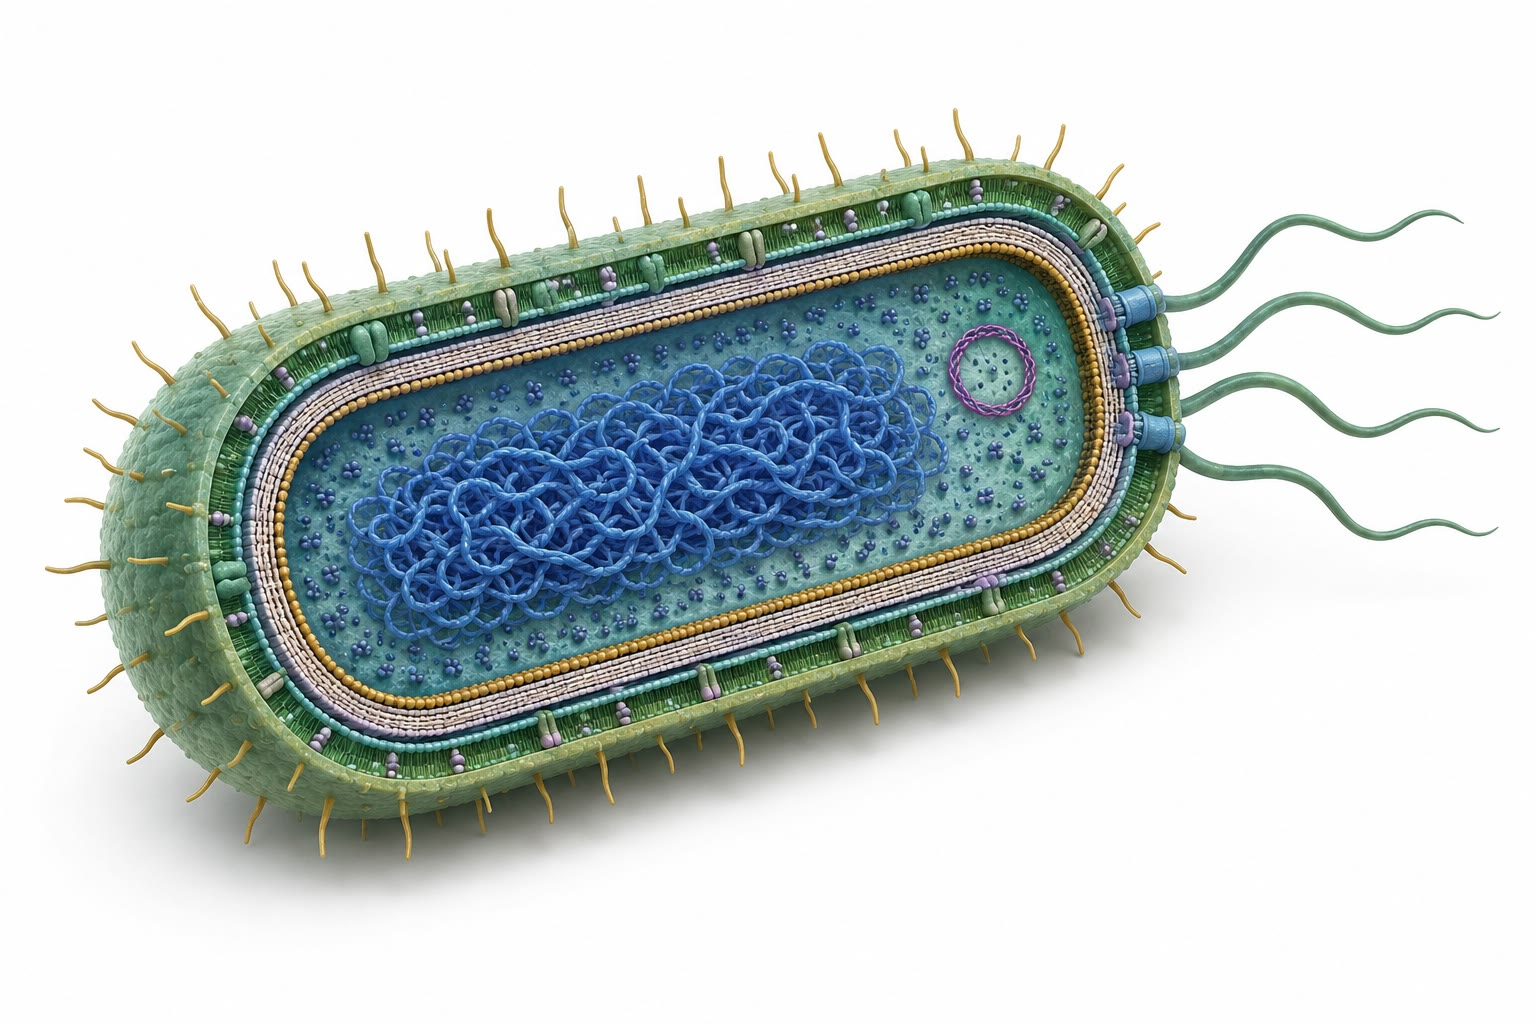
\includegraphics[width=0.54\linewidth]{images/book3/ai/fig-ecoli-cell.jpg}};
  \begin{scope}[x={(img.south east)}, y={(img.north west)},
      every node/.style={font=\small}]
    \draw[omDef, thick] (0.45,0.52) -- (0.45,1.08) node[above] {nucleoïde: ringvormig DNA};
    \draw[omDef, thick] (0.75,0.55) -- (1.03,0.46) node[right] {ribosomen};
    \draw[omDef, thick] (0.17,0.45) -- (-0.03,0.40) node[left, align=right] {wand en\\ twee membranen};
    \draw[omDef, thick] (0.65,0.64) -- (1.03,0.24) node[right] {plasmide};
    \draw[omDef, thick] (0.88,0.68) -- (1.03,0.80) node[right] {flagellen};
    \draw[omDef, thick] (0.35,0.19) -- (0.35,-0.08) node[below] {pili};
  \end{scope}
\end{tikzpicture}

{\small Een bacterie (\emph{Escherichia coli}), opengesneden. Geen kern, geen
\omterm{def:b1:cell-unit-of-life:prokeuk}{organellen}: een ringvormig chromosoom los opgevouwen in het \omterm{def:b1:cell-unit-of-life:cell}{cytoplasma} tussen
duizenden ribosomen, een wand buiten de \omterm{def:b1:cell-unit-of-life:cell}{plasmamembraan}, flagellen om te zwemmen
en pili om zich te hechten. Lengte ongeveer \qty{2}{\micro m}.}
\end{omfigure}

\begin{omfigure}
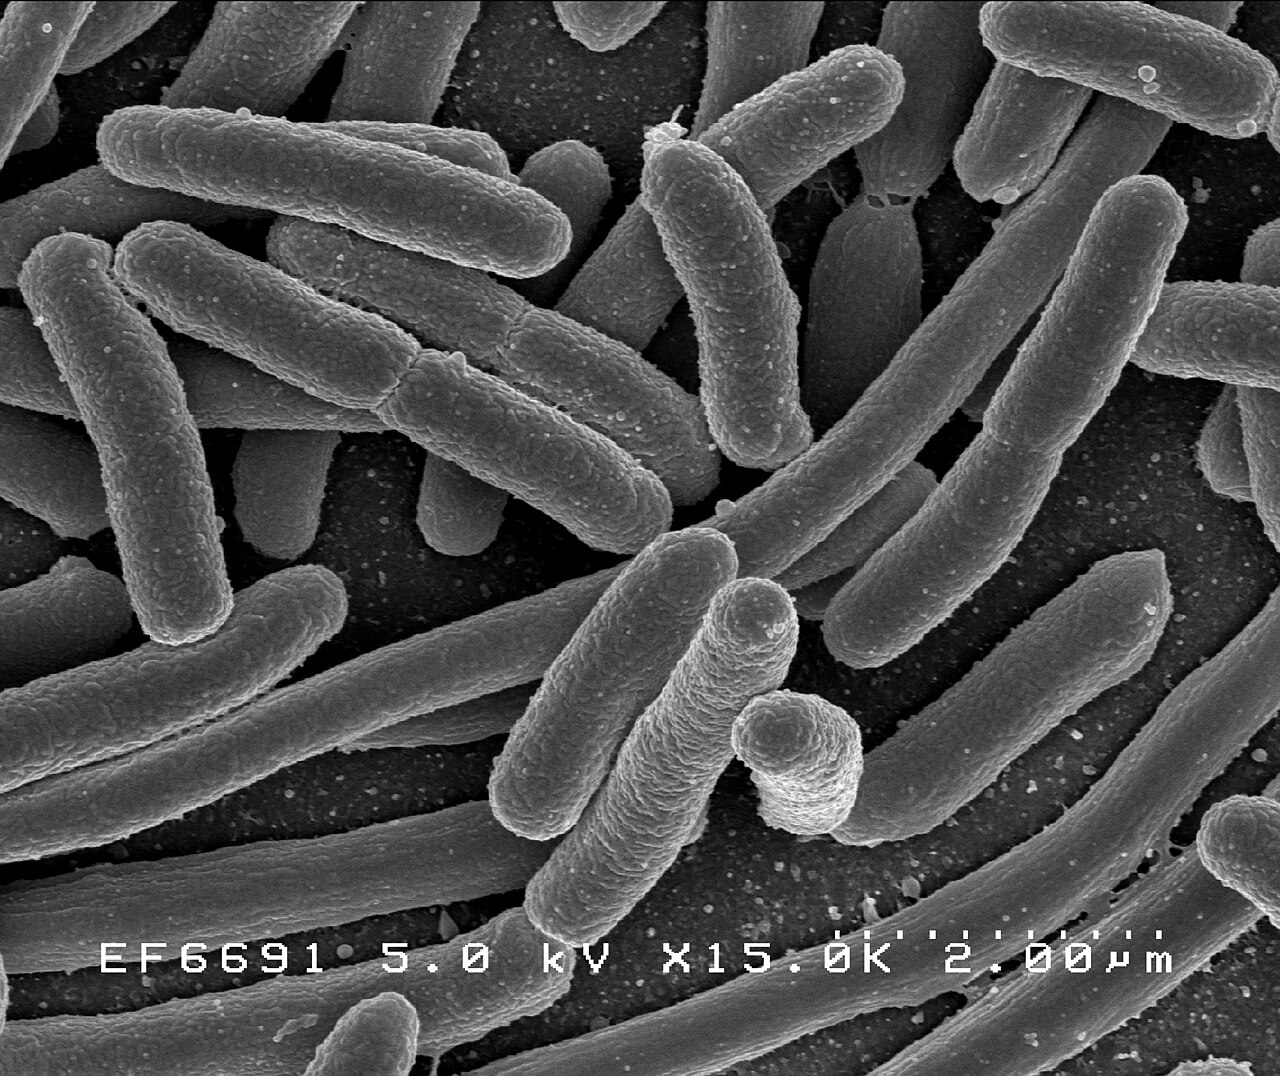
\includegraphics[width=0.5\linewidth]{images/book3/ecoli-niaid.jpg}

{\small \emph{Escherichia coli} onder de rasterelektronenmicroscoop (het
streepje onderaan het beeld is \qty{2}{\micro m}). Staafjes van
\qty{2}{\micro m} lang, waarvan er duizend naast elkaar op een millimeter
passen; één \omterm{def:b1:cell-unit-of-life:cell}{cel} deelt in een rijk medium elke twintig minuten. Beeld: NIAID,
publiek domein.}
\end{omfigure}

\begin{proposition}[De bacteriecel]\label{prop:b1:cell-unit-of-life:bacterium}
\emph{E. coli}, de modelbacterie, is een staafje van \qty{2}{\micro m} lang en
\qty{0.8}{\micro m} breed: een volume van ongeveer \qty{1}{\micro m^3} met daarin
één chromosoom van $\num{4.6e6}$ basenparen (\qty{1.5}{mm} DNA, tienduizendvoudig
opgevouwen), zo'n \num{20000} ribosomen, enkele miljoenen eiwitmoleculen van
\num{2000} soorten, en vaak een of meer
\emph{plasmiden}\index{plasmide} --- kleine ringvormige DNA-moleculen met extra
genen. Haar omhulsel bestaat, van binnen naar buiten, uit de \omterm{def:b1:cell-unit-of-life:cell}{plasmamembraan}, een
dunne wand van \emph{peptidoglycaan}\index{peptidoglycaan} (een netwerk van
suikerketens dwarsverbonden door korte peptiden, dat de inwendige druk van de \omterm{def:b1:cell-unit-of-life:cell}{cel}
weerstaat), en een buitenmembraan. Bacteriën met een dikke peptidoglycaanwand en
zonder buitenmembraan houden de kristalvioletkleuring van de
\emph{gramkleuring}\index{gramkleuring} vast (grampositief); die met een dunne
wand onder een buitenmembraan verliezen haar (gramnegatief, zoals
\emph{E. coli}). Flagellen draaien als schroeven; pili hechten de \omterm{def:b1:cell-unit-of-life:cell}{cel} aan
oppervlakken en aan andere \omterm{def:b1:cell-unit-of-life:cell}{cellen}.
\end{proposition}

\begin{method}[De gramkleuring]\label{met:b1:cell-unit-of-life:gram}
\begin{enumerate}
  \item Fixeer een dun uitstrijkje bacteriën met warmte op een glaasje.
  \item Kleur met kristalviolet (alle \omterm{def:b1:cell-unit-of-life:cell}{cellen} paars) en vervolgens met
        jodium, dat binnen de \omterm{def:b1:cell-unit-of-life:cell}{cellen} een groot complex met de kleurstof
        vormt.
  \item Spoel met alcohol: het dikke peptidoglycaan van grampositieve
        \omterm{def:b1:cell-unit-of-life:cell}{cellen} krimpt en houdt het complex vast; de dunne wand van
        gramnegatieve \omterm{def:b1:cell-unit-of-life:cell}{cellen} laat het uitspoelen zodra de alcohol de
        buitenmembraan heeft opgelost.
  \item Kleur na met een roze kleurstof (safranine): grampositieve \omterm{def:b1:cell-unit-of-life:cell}{cellen}
        zien er paars uit, gramnegatieve roze. De uitslag voorspelt de
        bouw van de wand en daarmee de gevoeligheid voor veel
        antibiotica.
\end{enumerate}
\end{method}

\begin{omfigure}
\begin{tikzpicture}
\begin{semilogxaxis}[
  width=0.94\linewidth, height=6.0cm,
  axis x line=bottom, axis y line=none,
  xmin=0.05, xmax=5000000, ymin=0, ymax=1.6,
  xlabel={grootte (\unit{nm})},
  xlabel style={font=\small, at={(axis description cs:0.5,-0.14)}, anchor=north},
  xtick={0.1,1,10,100,1000,10000,100000,1000000}, log ticks with fixed point,
  xticklabels={0.1,1,10,100,\qty{1}{\micro m},\qty{10}{\micro m},\qty{100}{\micro m},\qty{1}{mm}},
  tick label style={font=\small}, clip=false,
]
\addplot[only marks, mark=*, mark size=1.8pt, omDef] coordinates {(0.1,0.75) (1,0.75) (10,0.75) (30,0.75) (100,0.75) (1000,0.75) (4000,0.75) (20000,0.75) (100000,0.75) (1000000,0.75)};
\node[font=\scriptsize, anchor=west, rotate=65, inner sep=1pt] at (axis cs:0.1,0.82) {atoom};
\node[font=\scriptsize, anchor=west, rotate=65, inner sep=1pt] at (axis cs:1,0.82) {glucose};
\node[font=\scriptsize, anchor=west, rotate=65, inner sep=1pt] at (axis cs:10,0.82) {eiwit};
\node[font=\scriptsize, anchor=west, rotate=65, inner sep=1pt] at (axis cs:30,0.82) {ribosoom};
\node[font=\scriptsize, anchor=west, rotate=65, inner sep=1pt] at (axis cs:100,0.82) {virus};
\node[font=\scriptsize, anchor=west, rotate=65, inner sep=1pt] at (axis cs:1000,0.82) {bacterie};
\node[font=\scriptsize, anchor=west, rotate=65, inner sep=1pt] at (axis cs:4000,0.82) {mitochondrion};
\node[font=\scriptsize, anchor=west, rotate=65, inner sep=1pt] at (axis cs:20000,0.82) {dierlijke cel};
\node[font=\scriptsize, anchor=west, rotate=65, inner sep=1pt] at (axis cs:100000,0.82) {menselijke eicel};
\node[font=\scriptsize, anchor=west, rotate=65, inner sep=1pt] at (axis cs:1000000,0.82) {kikkerei};
\draw[very thick, omThm] (axis cs:0.2,0.52) -- (axis cs:1000000,0.52) node[pos=0.5, above, font=\scriptsize, omThm, inner sep=1.5pt] {elektronenmicroscoop};
\draw[very thick, omProp] (axis cs:200,0.34) -- (axis cs:1000000,0.34) node[pos=0.5, above, font=\scriptsize, omProp, inner sep=1.5pt] {lichtmicroscoop};
\draw[very thick, omExo] (axis cs:100000,0.16) -- (axis cs:5000000,0.16) node[pos=0.5, above, font=\scriptsize, omExo, inner sep=1.5pt] {blote oog};
\end{semilogxaxis}
\end{tikzpicture}

{\small De afmetingen van de dingen, op een logaritmische schaal, en de
instrumenten die ze scheiden. Bacteriën liggen net boven de grens van de
\omterm{prop:b1:cell-unit-of-life:microscopes}{lichtmicroscoop}; de \omterm{def:b1:cell-unit-of-life:prokeuk}{eukaryote cel} is in elke richting tien keer groter, in
volume duizend keer.}
\end{omfigure}

\begin{example}[Waarom de eukaryote cel gecompartimenteerd is]\label{ex:b1:cell-unit-of-life:whycompart}
Een \omterm{def:b1:cell-unit-of-life:cell}{cel} van \qty{20}{\micro m} heeft duizend keer het volume van een bacterie,
maar slechts honderd keer haar membraanoppervlak
(\cref{prop:b1:organism-environment:sv}). Membranen zijn de plaats waar een \omterm{def:b1:cell-unit-of-life:cell}{cel}
haar energieomzettende ketens en haar transportsystemen draagt; de eukaryoot
wint oppervlak terug door membranen in zichzelf te vouwen --- het binnenmembraan
van een mitochondrion, de bladen van het endoplasmatisch reticulum --- en wint
daarbovenop afzonderlijke kamers waarin onverenigbare chemie (vertering in het
lysosoom, opbouw in het cytosol) naast elkaar kan verlopen.
\end{example}

\section{Cellen zien: microscopie}

\begin{definition}[Vergroting en oplossend vermogen]\label{def:b1:cell-unit-of-life:resolution}
Een microscoop \emph{vergroot}\index{vergroting} (maakt het beeld groter) en
\emph{scheidt}\index{resolutie} (houdt naburige punten uit elkaar). Alleen het
tweede begrenst wat er te zien is: het \emph{oplossend
vermogen}\index{oplossend vermogen} is de kleinste afstand $d$ tussen twee
punten die nog afzonderlijk zichtbaar zijn,
\[
d = \frac{0.61\,\lambda}{\mathrm{NA}},
\]
waarin $\lambda$ de golflengte van de belichting is en $\mathrm{NA}$ de
numerieke apertuur van het objectief (de sinus van zijn halve openingshoek maal
de brekingsindex van het medium, hoogstens ongeveer $1.4$ met olie). Verder
vergroten dan het oplossend vermogen vergroot de vaagheid en niet het detail.
\end{definition}

\begin{proposition}[Licht- en elektronenmicroscopen]\label{prop:b1:cell-unit-of-life:microscopes}
Met zichtbaar licht ($\lambda \approx \qty{550}{nm}$) en $\mathrm{NA} = 1.4$
scheidt de \emph{lichtmicroscoop}\index{lichtmicroscoop} \qty{0.24}{\micro m}:
\omterm{def:b1:cell-unit-of-life:cell}{cellen}, kernen, chloroplasten, mitochondriën als stipjes, bacteriën als
staafjes --- en levende, bewegende preparaten. Contrast in een doorzichtige \omterm{def:b1:cell-unit-of-life:cell}{cel}
wordt verkregen door kleuring (die meestal doodt), door \emph{fasecontrast}
(dat verschillen in brekingsindex in verschillen in helderheid omzet), of door
\emph{fluorescentie} (waarbij één molecuul met een kleurstof of een fluorescerend
eiwit wordt gemerkt en alleen zijn licht wordt afgebeeld). De
\emph{elektronenmicroscoop}\index{elektronenmicroscoop} gebruikt elektronen met
een golflengte van enkele picometers; zijn praktische \omterm{def:b1:cell-unit-of-life:resolution}{oplossend vermogen}, begrensd
door zijn lenzen, is ongeveer \qty{0.2}{nm} in transmissie (TEM: elektronen gaan
door een coupe van \qty{50}{nm} dik die met zware metalen is gekleurd, en geven de
inwendige bouw van \omterm{def:b1:cell-unit-of-life:prokeuk}{organellen}) en enkele nanometers bij rastering (SEM: een bundel
die over een met metaal bedekt oppervlak wordt gestreken en het reliëf in de
diepte geeft). Elektronenmicroscopie vereist vacuüm en dode, gefixeerde,
gedroogde preparaten.
\end{proposition}

\begin{omfigure}
\begin{tikzpicture}[font=\footnotesize, >=Stealth, line cap=round]
  % optical axis
  \draw[gray, dashed] (0,0) -- (11.4,0);
  % object
  \draw[very thick, omExo, ->] (0.6,0) -- (0.6,0.35) node[above, font=\scriptsize] {voorwerp};
  % objective lens
  \draw[very thick, omDef] (2.0,-0.9) .. controls (2.35,0) .. (2.0,0.9);
  \draw[very thick, omDef] (2.0,-0.9) .. controls (1.65,0) .. (2.0,0.9);
  \node[below, font=\scriptsize] at (2.0,-1.0) {objectief};
  % intermediate image
  \draw[very thick, omExo, ->] (6.2,0) -- (6.2,-1.4) node[below, font=\scriptsize] {tussenbeeld (omgekeerd, vergroot)};
  % eyepiece
  \draw[very thick, omDef] (8.4,-0.9) .. controls (8.75,0) .. (8.4,0.9);
  \draw[very thick, omDef] (8.4,-0.9) .. controls (8.05,0) .. (8.4,0.9);
  \node[above, font=\scriptsize] at (8.4,1.0) {oculair};
  % eye
  \draw[thick] (10.6,0) circle (0.35); \node[font=\scriptsize, above] at (10.6,0.45) {oog};
  % rays: from object tip through objective to image tip
  \draw[omThm, thick] (0.6,0.35) -- (2.0,0.35) -- (6.2,-1.4);
  \draw[omThm, thick] (0.6,0.35) -- (2.0,-0.55) -- (6.2,-1.4);
  % rays from image tip through eyepiece, emerging parallel (virtual image at infinity)
  \draw[omThm, thick] (6.2,-1.4) -- (8.4,-0.6) -- (10.3,-0.15);
  \draw[omThm, thick] (6.2,-1.4) -- (8.4,0.5) -- (10.3,0.25);
  \node[align=center, font=\scriptsize, gray] at (4.2,1.2) {vergroting = objectief $\times$ oculair\\ bv.\ $100\times$ olie-objectief $\times 10\times$ oculair $= 1000\times$};
\end{tikzpicture}

{\small De samengestelde \omterm{prop:b1:cell-unit-of-life:microscopes}{lichtmicroscoop}: het objectief vormt een \omterm{def:b1:cell-unit-of-life:resolution}{vergroot},
omgekeerd tussenbeeld, dat het oculair nog eens \omterm{def:b1:cell-unit-of-life:resolution}{vergroot} voor het oog. De
numerieke apertuur van het objectief, en niet de totale \omterm{def:b1:cell-unit-of-life:resolution}{vergroting}, bepaalt wat
er te scheiden valt.}
\end{omfigure}

\begin{omfigure}
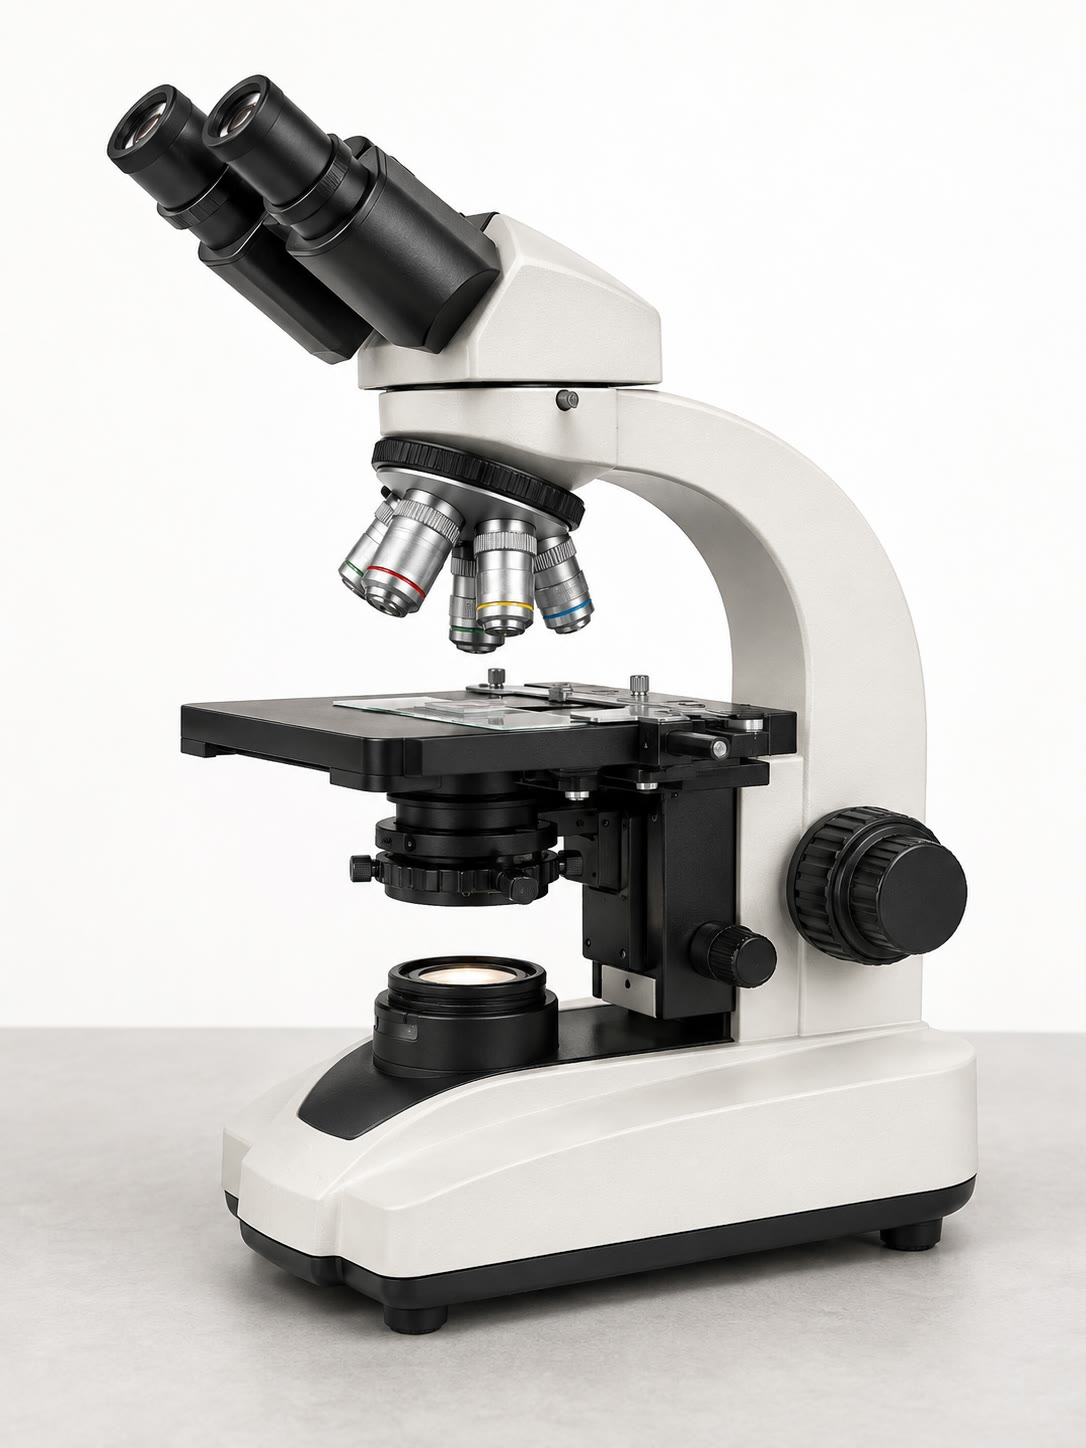
\includegraphics[width=0.36\linewidth]{images/book3/ai/b3-05-light-microscope.jpg}

{\small Een samengestelde \omterm{prop:b1:cell-unit-of-life:microscopes}{lichtmicroscoop}: lamp en condensor onder de tafel, een
revolver met objectieven erboven, binoculaire oculairen. \omterm{def:b1:cell-unit-of-life:resolution}{Oplossend vermogen}
\qty{0.2}{\micro m}, \omterm{def:b1:cell-unit-of-life:resolution}{vergroting} tot \qty{1000}{}, levende preparaten mogelijk.}
\end{omfigure}

\begin{method}[Het instrument kiezen]\label{met:b1:cell-unit-of-life:choose}
\begin{enumerate}
  \item Om een levend proces te volgen (celdeling, beweging, een
        fluorescerend eiwit dat tussen compartimenten verhuist):
        lichtmicroscopie, fasecontrast of fluorescentie, op ongefixeerde
        \omterm{def:b1:cell-unit-of-life:cell}{cellen}.
  \item Om \omterm{def:b1:cell-unit-of-life:cell}{cellen} in een \omterm{def:b1:body-plans-tissues:tissue}{weefsel} te tellen en te herkennen: een
        gefixeerd, gesneden, gekleurd preparaat onder de \omterm{prop:b1:cell-unit-of-life:microscopes}{lichtmicroscoop}.
  \item Om de inwendige bouw van een \omterm{def:b1:cell-unit-of-life:prokeuk}{organel}, een membraan of een virus
        te zien: transmissie-elektronenmicroscopie van dunne coupes, of
        van negatief gekleurde deeltjes.
  \item Om het oppervlaktereliëf van een \omterm{def:b1:cell-unit-of-life:cell}{cel} of een \omterm{def:b1:body-plans-tissues:tissue}{weefsel} te zien:
        raster\-elektronenmicroscopie.
  \item Om één eiwit te lokaliseren: immunofluorescentie (licht) of
        immunogoudmerking (elektronen), met een antistof ertegen.
\end{enumerate}
\end{method}

\begin{example}[Een bacterie en een mitochondrion]\label{ex:b1:cell-unit-of-life:seeing}
Onder de \omterm{prop:b1:cell-unit-of-life:microscopes}{lichtmicroscoop} bij $1000\times$ is een \omterm{def:b1:cell-unit-of-life:cell}{cel} van \emph{E. coli} op de
schaal van het netvlies een staafje van \qty{2}{mm} lang, zonder zichtbare
binnenkant; een mitochondrion is een stip op de grens van het \omterm{def:b1:cell-unit-of-life:resolution}{oplossend
vermogen}. In een TEM-coupe toont dezelfde bacterie haar twee membranen, haar
wand, haar \omterm{def:b1:cell-unit-of-life:prokeuk}{nucleoïde} als een bleek vezelig gebied en haar ribosomen als donkere
korrels; het mitochondrion toont zijn dubbele membraan en de plooien van het
binnenste. Geen van beide leeft nog.
\end{example}

\section{Cellen uit elkaar halen en in leven houden}

\begin{definition}[Celfractionering]\label{def:b1:cell-unit-of-life:fractionation}
\emph{Celfractionering}\index{celfractionering} scheidt de onderdelen van een \omterm{def:b1:cell-unit-of-life:cell}{cel}
voor nader onderzoek. Het \omterm{def:b1:body-plans-tissues:tissue}{weefsel} wordt
\emph{gehomogeniseerd}\index{homogenaat} --- de \omterm{def:b1:cell-unit-of-life:cell}{cellen} worden in een koude,
isotone buffer opengebroken door malen of afschuiven, waarbij de \omterm{def:b1:cell-unit-of-life:prokeuk}{organellen} heel
blijven --- en het homogenaat wordt onderworpen aan \emph{differentiële
centrifugatie}\index{differentiële centrifugatie}: een reeks slingerbeurten met
toenemende kracht en duur, die telkens de grootste en dichtste deeltjes die nog
in suspensie zijn tot een pellet slaat. Elke fractie wordt herkend aan haar
aanblik onder de \omterm{prop:b1:cell-unit-of-life:microscopes}{elektronenmicroscoop} en aan
\emph{merkerenzymen}\index{merkerenzym}, activiteiten waarvan bekend is dat zij
in slechts één compartiment thuishoren.
\end{definition}

\begin{omfigure}
\begin{tikzpicture}[font=\footnotesize, >=Stealth, line cap=round,
  tube/.style={draw, thick, rounded corners=2pt, minimum width=20mm, minimum height=9mm, align=center, fill=white},
  pel/.style={draw, thick, rounded corners=3pt, text width=29mm, minimum height=10mm, align=center, fill=omProp!15}]
  \node[tube, fill=omDef!10] (h) at (0,0) {homogenaat};
  \node[tube, fill=omDef!10] (s1) at (3.5,0) {supernatant 1};
  \node[tube, fill=omDef!10] (s2) at (7.0,0) {supernatant 2};
  \node[tube, fill=omDef!10] (s3) at (10.5,0) {supernatant 3};
  \node[tube, fill=omExo!15] (cy) at (13.6,0) {cytosol};
  \draw[->, thick] (h) -- (s1) node[midway, above, align=center, font=\scriptsize] {$1000\,g$\\ \qty{10}{min}};
  \draw[->, thick] (s1) -- (s2) node[midway, above, align=center, font=\scriptsize] {$\num{10000}\,g$\\ \qty{20}{min}};
  \draw[->, thick] (s2) -- (s3) node[midway, above, align=center, font=\scriptsize] {$\num{100000}\,g$\\ \qty{60}{min}};
  \draw[->, thick] (s3) -- (cy) node[midway, above, align=center, font=\scriptsize] {geen\\ pellet};
  \node[pel] (p1) at (1.75,-1.9) {pellet 1: kernen, hele cellen, resten};
  \node[pel] (p2) at (5.25,-1.9) {pellet 2: mitochondriën, lysosomen, peroxisomen};
  \node[pel] (p3) at (8.75,-1.9) {pellet 3: microsomen (ER-fragmenten), ribosomen};
  \draw[->, thick] (1.75,-0.5) -- (p1);
  \draw[->, thick] (5.25,-0.5) -- (p2);
  \draw[->, thick] (8.75,-0.5) -- (p3);
  \node[align=left, gray, anchor=north west, font=\scriptsize] at (10.4,-1.3) {merkers: DNA (kernen),\\ succinaatdehydrogenase\\ (mitochondriën), zure\\ fosfatase (lysosomen),\\ glucose-6-fosfatase (ER),\\ lactaatdehydrogenase (cytosol)};
\end{tikzpicture}

{\small \omterm{def:b1:cell-unit-of-life:fractionation}{Differentiële centrifugatie} van een \omterm{def:b1:cell-unit-of-life:fractionation}{homogenaat}. Elke slingerbeurt slaat
neer wat groter of dichter is dan wat de vorige in suspensie liet: eerst de
kernen, dan de mitochondriën, dan de membraanfragmenten, en ten slotte het
oplosbare cytosol. \omterm{def:b1:cell-unit-of-life:fractionation}{Merkerenzymen} vertellen welk \omterm{def:b1:cell-unit-of-life:prokeuk}{organel} waar terechtkwam.}
\end{omfigure}

\begin{omfigure}
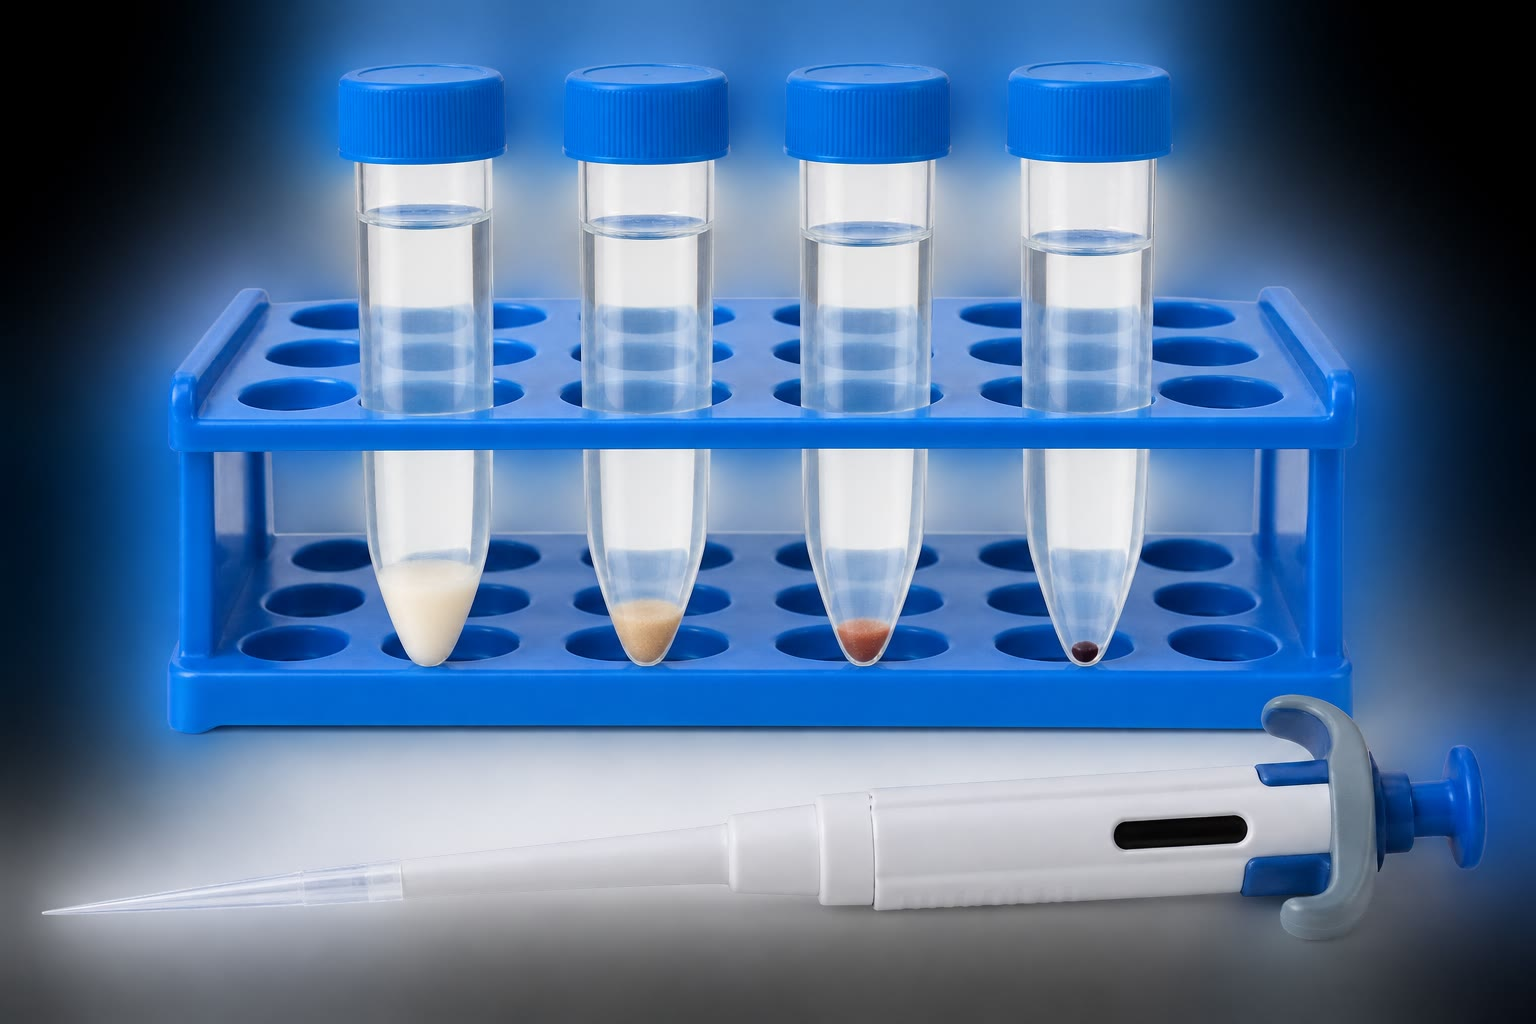
\includegraphics[width=0.5\linewidth]{images/book3/ai/b3-05-fractionation-tubes.jpg}

{\small Fracties na opeenvolgende slingerbeurten: de pellets van kernen,
mitochondriën en microsomen, elk onder zijn opgehelderde supernatant.}
\end{omfigure}

\begin{proposition}[Sedimentatie]\label{prop:b1:cell-unit-of-life:stokes}
Een bolvormig deeltje met straal $r$ en dichtheid $\rho_p$ in een vloeistof met
dichtheid $\rho_f$ en viscositeit $\eta$, in een middelpuntvliedend veld $g_c$
(een veelvoud van $g$), sedimenteert met de constante snelheid
\[
v = \frac{2}{9}\,\frac{r^2\,(\rho_p - \rho_f)\,g_c}{\eta}
\]
(de wet van Stokes). De snelheid groeit met het kwadraat van de straal: een kern
van \qty{5}{\micro m} valt honderd keer sneller dan een mitochondrion van
\qty{0.5}{\micro m}, dat weer duizend keer sneller valt dan een ribosoom van
\qty{15}{nm}. Daarom scheidt dezelfde buis ze bij toenemende toerentallen.
\end{proposition}
\begin{proof}
Bij constante snelheid is de wrijvingskracht van Stokes, $6\pi\eta r v$, in
evenwicht met het netto gewicht van het deeltje in de vloeistof,
$\frac{4}{3}\pi r^3(\rho_p - \rho_f)g_c$; oplossen naar $v$ geeft de formule.
\end{proof}

\begin{definition}[Celkweek]\label{def:b1:cell-unit-of-life:culture}
\emph{Celkweek}\index{celkweek} houdt \omterm{def:b1:cell-unit-of-life:cell}{cellen} buiten het \omterm{def:b1:organism-environment:organism}{organisme} in leven en aan
het delen, in een steriel medium dat voedingsstoffen, zouten, groeifactoren en,
voor dierlijke \omterm{def:b1:cell-unit-of-life:cell}{cellen}, een oppervlak om aan te hechten levert, op de temperatuur
van het \omterm{def:b1:organism-environment:organism}{organisme}. Bacteriën en gisten groeien in eenvoudige media en verdubbelen
in minuten tot uren; dierlijke \omterm{def:b1:cell-unit-of-life:cell}{cellen} die rechtstreeks uit een \omterm{def:b1:body-plans-tissues:tissue}{weefsel} komen
(\emph{primaire kweken}) delen een beperkt aantal keren, terwijl
\emph{cellijnen} afkomstig van tumoren of getransformeerde \omterm{def:b1:cell-unit-of-life:cell}{cellen} zich onbeperkt
delen. De kweek maakt van de \omterm{def:b1:cell-unit-of-life:cell}{cel} een experimenteel object: één celtype, één
medium, één variabele tegelijk.
\end{definition}

\begin{example}[Een groeicurve]\label{ex:b1:cell-unit-of-life:growthcurve}
Een kolf \emph{E. coli} in een rijk medium bij \qty{37}{\celsius}: een
aanloopfase van een half uur, dan exponentiële groei --- het aantal verdubbelt
elke \qty{20}{min}, dus $N = N_0\,2^{t/20}$ --- tot een voedingsstof opraakt of
afvalstoffen zich ophopen en de kweek een plateau bereikt van bijna $10^9$ \omterm{def:b1:cell-unit-of-life:cell}{cellen}
per milliliter. Uit één \omterm{def:b1:cell-unit-of-life:cell}{cel} ontstaan in tien uur $2^{30} \approx 10^9$ \omterm{def:b1:cell-unit-of-life:cell}{cellen}.
Dezelfde curve, met een verdubbelingstijd van een dag, beschrijft een kweek van
menselijke \omterm{def:b1:cell-unit-of-life:cell}{cellen}.
\end{example}

\section{Opgaven}

\begin{exercise}[$\star$]\label{exo:b1:cell-unit-of-life:1}
Formuleer de drie uitspraken van de \omterm{prop:b1:cell-unit-of-life:theory}{celtheorie} en noem voor elk een stuk
bewijsmateriaal.
\end{exercise}

\begin{exercise}[$\star$]\label{exo:b1:cell-unit-of-life:2}
Noem vier verschillen tussen een prokaryote en een \omterm{def:b1:cell-unit-of-life:prokeuk}{eukaryote cel}.
\end{exercise}

\begin{exercise}[$\star$]\label{exo:b1:cell-unit-of-life:3}
Hoeveel bacteriën, op een rij gelegd, overbruggen volgens de figuur van de
groottes een kikkerei? Hoeveel dierlijke \omterm{def:b1:cell-unit-of-life:cell}{cellen}?
\end{exercise}

\begin{exercise}[$\star$]\label{exo:b1:cell-unit-of-life:4}
Waarom toont een \omterm{prop:b1:cell-unit-of-life:microscopes}{lichtmicroscoop} bij $2000\times$ niet meer detail dan een bij
$1000\times$?
\end{exercise}

\begin{exercise}[$\star\star$]\label{exo:b1:cell-unit-of-life:5}
Bereken het \omterm{def:b1:cell-unit-of-life:resolution}{oplossend vermogen} van een objectief met $\mathrm{NA} = 0.65$ in
groen licht (\qty{550}{nm}) en in blauw licht (\qty{450}{nm}). Kan het twee
bacteriën op \qty{0.5}{\micro m} van elkaar scheiden? En twee ribosomen op
\qty{30}{nm}?
\end{exercise}

\begin{exercise}[$\star\star$]\label{exo:b1:cell-unit-of-life:6}
Een \omterm{prop:b1:cell-unit-of-life:bacterium}{gramkleuring} van een gemengde kweek toont paarse kokken en roze staafjes.
Wat zegt elke kleur over de \omterm{def:b1:cell-unit-of-life:prokeuk}{celwand}? Welke van de twee is \emph{E. coli}?
\end{exercise}

\begin{exercise}[$\star\star$]\label{exo:b1:cell-unit-of-life:7}
Bereken met de wet van Stokes, met $\eta = \qty{1e-3}{Pa.s}$ en $\rho_p - \rho_f =
\qty{100}{kg/m^3}$, de sedimentatiesnelheid van een mitochondrion
($r = \qty{0.5}{\micro m}$) bij $\num{10000}\,g$ en de tijd om \qty{5}{cm} af te
leggen. Herhaal dat voor een kern ($r = \qty{4}{\micro m}$) bij $1000\,g$.
\end{exercise}

\begin{exercise}[$\star\star$]\label{exo:b1:cell-unit-of-life:8}
De merkeractiviteiten van een \omterm{def:b1:cell-unit-of-life:fractionation}{homogenaat} zijn: succinaatdehydrogenase
\qty{80}{\%} in pellet 2, \qty{15}{\%} in pellet 1, \qty{5}{\%} in het
supernatant; lactaatdehydrogenase \qty{95}{\%} in het laatste supernatant. Duid
elk getal, inclusief de \qty{15}{\%} in pellet 1.
\end{exercise}

\begin{exercise}[$\star\star$]\label{exo:b1:cell-unit-of-life:9}
Welke microscoop zou je gebruiken om (a) een witte bloedcel een bacterie te zien
opslokken, (b) de mitochondriën in een coupe spier te tellen, (c) de poriën van
een kernenvelop te zien, (d) de vorm van het oppervlak van een stuifmeelkorrel te
zien? Verantwoord elke keuze.
\end{exercise}

\begin{exercise}[$\star\star\star$]\label{exo:b1:cell-unit-of-life:10}
De kolven van Pasteur: een bouillon die in een zwanenhalskolf is gekookt blijft
onbeperkt helder; kantelt men de kolf zodat de bouillon het stof in de hals
raakt, dan wordt zij binnen twee dagen troebel. Leg uit wat elke waarneming
uitsluit en wat het paar bewijst, en zeg waarom koken in een afgesloten kolf op
zichzelf de vraag niet had beslecht.
\end{exercise}

\begin{exercise}[$\star\star\star$]\label{exo:b1:cell-unit-of-life:11}
Een kweek van \emph{E. coli} begint met $10^3$ \omterm{def:b1:cell-unit-of-life:cell}{cellen} per milliliter en
verdubbelt elke \qty{25}{min}. Wanneer bereikt zij $10^8$ per milliliter? Als
elke \omterm{def:b1:cell-unit-of-life:cell}{cel} een massa van \qty{1}{pg} heeft, hoeveel bacteriemassa zit er dan op dat
moment in een liter, en waarom stopt de groei kort daarna, zelfs bij een
overmaat glucose?
\end{exercise}

\begin{exercise}[$\star\star\star$]\label{exo:b1:cell-unit-of-life:12}
``De \omterm{def:b1:cell-unit-of-life:prokeuk}{eukaryote cel} is een bacterie die heeft leren vouwen.'' Bespreek dat in een
alinea, aan de hand van de verhouding tussen oppervlak en volume, de membranen
van \omterm{def:b1:cell-unit-of-life:prokeuk}{organellen}, en wat compartimenten mogelijk maken.
\end{exercise}

\section{Vraagstuk: een lever fractioneren}

\begin{problem}[{Weekendvraagstuk --- tien gram rattenlever uit elkaar gehaald
door centrifugatie: pellets, merkers, de wet van Stokes en de balans van een
enzym, eindigend op de zuiveringsfactor van de mitochondriale fractie}]
\label{pb:b1:cell-unit-of-life:1}
\qty{10}{g} rattenlever wordt \omterm{def:b1:cell-unit-of-life:fractionation}{gehomogeniseerd} in \qty{50}{mL} koude isotone
sucrose en in drie stappen geslingerd: $1000\,g$ gedurende \qty{10}{min}
(pellet 1), $\num{10000}\,g$ gedurende \qty{20}{min} (pellet 2),
$\num{100000}\,g$ gedurende \qty{60}{min} (pellet 3), waarna het laatste
supernatant overblijft. Het eiwitgehalte en twee enzymactiviteiten worden gemeten
in het \omterm{def:b1:cell-unit-of-life:fractionation}{homogenaat} en in elke fractie:

\begin{center}
\small
\begin{tabular}{lccc}
\hline
fractie & eiwit (mg) & succinaatdehydrogenase (U) & lactaatdehydrogenase (U) \\
\hline
\omterm{def:b1:cell-unit-of-life:fractionation}{homogenaat} & 2000 & 100 & 400 \\
pellet 1 & 500 & 15 & 20 \\
pellet 2 & 200 & 60 & 12 \\
pellet 3 & 300 & 5 & 8 \\
laatste supernatant & 950 & 4 & 350 \\
\hline
\end{tabular}
\end{center}

Neem $\eta = \qty{1e-3}{Pa.s}$ voor het medium, een sedimentatieweg van
\qty{5}{cm}, en $g = \qty{9.81}{m/s^2}$.

\medskip
\noindent\textbf{Deel I --- Wat waar zit.}
\begin{enumerate}
  \item Noem het belangrijkste \omterm{def:b1:cell-unit-of-life:prokeuk}{organel} in elke pellet.
  \item Waarom moet het homogenisatiemedium koud en isotoon zijn?
  \item Succinaatdehydrogenase is een merker van welk compartiment? En
        lactaatdehydrogenase van welk?
  \item Bereken de terugvinding van het eiwit: de som over de fracties als
        percentage van het \omterm{def:b1:cell-unit-of-life:fractionation}{homogenaat}. Becommentarieer dat.
  \item Bereken op dezelfde manier de terugvinding van elke
        enzymactiviteit.
  \item Bereken het eiwitgehalte per gram lever en de fractie van de verse
        massa van de lever die uit eiwit bestaat.
\end{enumerate}

\medskip
\noindent\textbf{Deel II --- De wet van Stokes.}
Mitochondriën: straal \qty{0.5}{\micro m}, dichtheidsoverschot
\qty{100}{kg/m^3}. Kernen: straal \qty{4}{\micro m}, hetzelfde overschot.
Ribosomen: straal \qty{12}{nm}, dichtheidsoverschot \qty{600}{kg/m^3}.
\begin{enumerate}[resume]
  \item Bereken de sedimentatiesnelheid van een mitochondrion bij
        $\num{10000}\,g$ en de tijd om \qty{5}{cm} af te leggen. Is
        \qty{20}{min} genoeg?
  \item Bereken de afstand die een mitochondrion tijdens de eerste
        slingerbeurt aflegt ($1000\,g$, \qty{10}{min}). Welk deel van de
        mitochondriën, bij aanvang gelijkmatig verdeeld, zou in de eerste
        stap worden neergeslagen?
  \item Vergelijk dat met de \qty{15}{\%} succinaatdehydrogenase die in
        pellet 1 wordt gevonden. Wat kan mitochondriën nog meer mee naar
        pellet 1 slepen?
  \item Bereken de tijd die een kern nodig heeft om bij $1000\,g$
        \qty{5}{cm} af te leggen.
  \item Bereken de tijd die een ribosoom nodig heeft om bij
        $\num{100000}\,g$ \qty{5}{cm} af te leggen. Zou een ribosoom bij
        $\num{10000}\,g$ in \qty{20}{min} worden neergeslagen?
  \item Leg uit waarom de reeks slingerbeurten oploopt in kracht en
        waarom elke stap lang genoeg maar niet te lang moet duren.
\end{enumerate}

\medskip
\noindent\textbf{Deel III --- Specifieke activiteit en zuivering.}
De specifieke activiteit van een enzym in een fractie is zijn activiteit per
milligram eiwit. De zuiveringsfactor van een fractie voor een enzym is zijn
specifieke activiteit gedeeld door die in het \omterm{def:b1:cell-unit-of-life:fractionation}{homogenaat}; de opbrengst is de
activiteit van de fractie gedeeld door die van het \omterm{def:b1:cell-unit-of-life:fractionation}{homogenaat}.
\begin{enumerate}[resume]
  \item Bereken de specifieke activiteit van succinaatdehydrogenase in het
        \omterm{def:b1:cell-unit-of-life:fractionation}{homogenaat} en in elke fractie.
  \item Bereken de zuiveringsfactor en de opbrengst van
        succinaatdehydrogenase in pellet 2.
  \item Bereken de zuiveringsfactor van succinaatdehydrogenase in
        pellet 3 en duid de waarde ervan.
  \item Bereken de specifieke activiteit van lactaatdehydrogenase in het
        \omterm{def:b1:cell-unit-of-life:fractionation}{homogenaat} en in het laatste supernatant, en de bijbehorende
        zuiveringsfactor en opbrengst.
  \item Waarom is de zuiveringsfactor van het cytosolische enzym lager dan
        die van het mitochondriale enzym, hoewel zijn opbrengst hoger is?
  \item Pellet 2 bevat \qty{12}{U} lactaatdehydrogenase. Is het enzym
        gedeeltelijk mitochondriaal? Stel een betere verklaring voor en
        een manier om die te toetsen.
  \item Welk deel van het levereiwit is mitochondriaal, als alle
        succinaatdehydrogenase mitochondriaal is en pellet 2 voor
        \qty{60}{\%} zuiver is? (Aanwijzing: gebruik de specifieke
        activiteit van zuivere mitochondriën, afgeleid uit pellet 2, en
        de totale activiteit.)
\end{enumerate}

\medskip
\noindent\textbf{Deel IV --- De fracties controleren.}
\begin{enumerate}[resume]
  \item Pellet 2 wordt met elektronenmicroscopie bekeken: welk instrument
        en welke bereiding, en wat zou er te zien moeten zijn?
  \item Hoe zou je pellet 1 op hele \omterm{def:b1:cell-unit-of-life:cell}{cellen} controleren, en wat zou je doen
        als je er veel vond?
  \item Pellet 2 wordt opnieuw in suspensie gebracht, op een
        sucrosedichtheidsgradiënt gelaagd en vervolgens geslingerd tot elk
        deeltje stilstaat waar zijn dichtheid gelijk is aan die van het
        medium. Mitochondriën vormen een band bij \qty{1.18}{g/mL},
        lysosomen bij \qty{1.22}{g/mL}, peroxisomen bij \qty{1.24}{g/mL}.
        Leg uit waarom deze scheiding werkt terwijl \omterm{def:b1:cell-unit-of-life:fractionation}{differentiële
        centrifugatie} haar niet tot stand kon brengen.
  \item De activiteit van zure fosfatase in pellet 2 stijgt scherp zodra
        er een detergens aan de bepaling wordt toegevoegd. Verklaar dat,
        en zeg wat het zegt over de toestand van de lysosomen in de
        pellet.
  \item Een student homogeniseert in zuiver water in plaats van in isotone
        sucrose. Voorspel het effect op pellet 2 en op de verdeling van
        succinaatdehydrogenase en zure fosfatase.
  \item Vat het resultaat samen: de zuiveringsfactor en de opbrengst van
        de mitochondriale fractie, en wat elk van beide begrenst.
\end{enumerate}
\end{problem}
